\chapter{Dynamic Routing}\label{dynamic-routing}

WHAT IS DYNAMIC ROUTING?

\begin{figure}
\centering
\pandocbounded{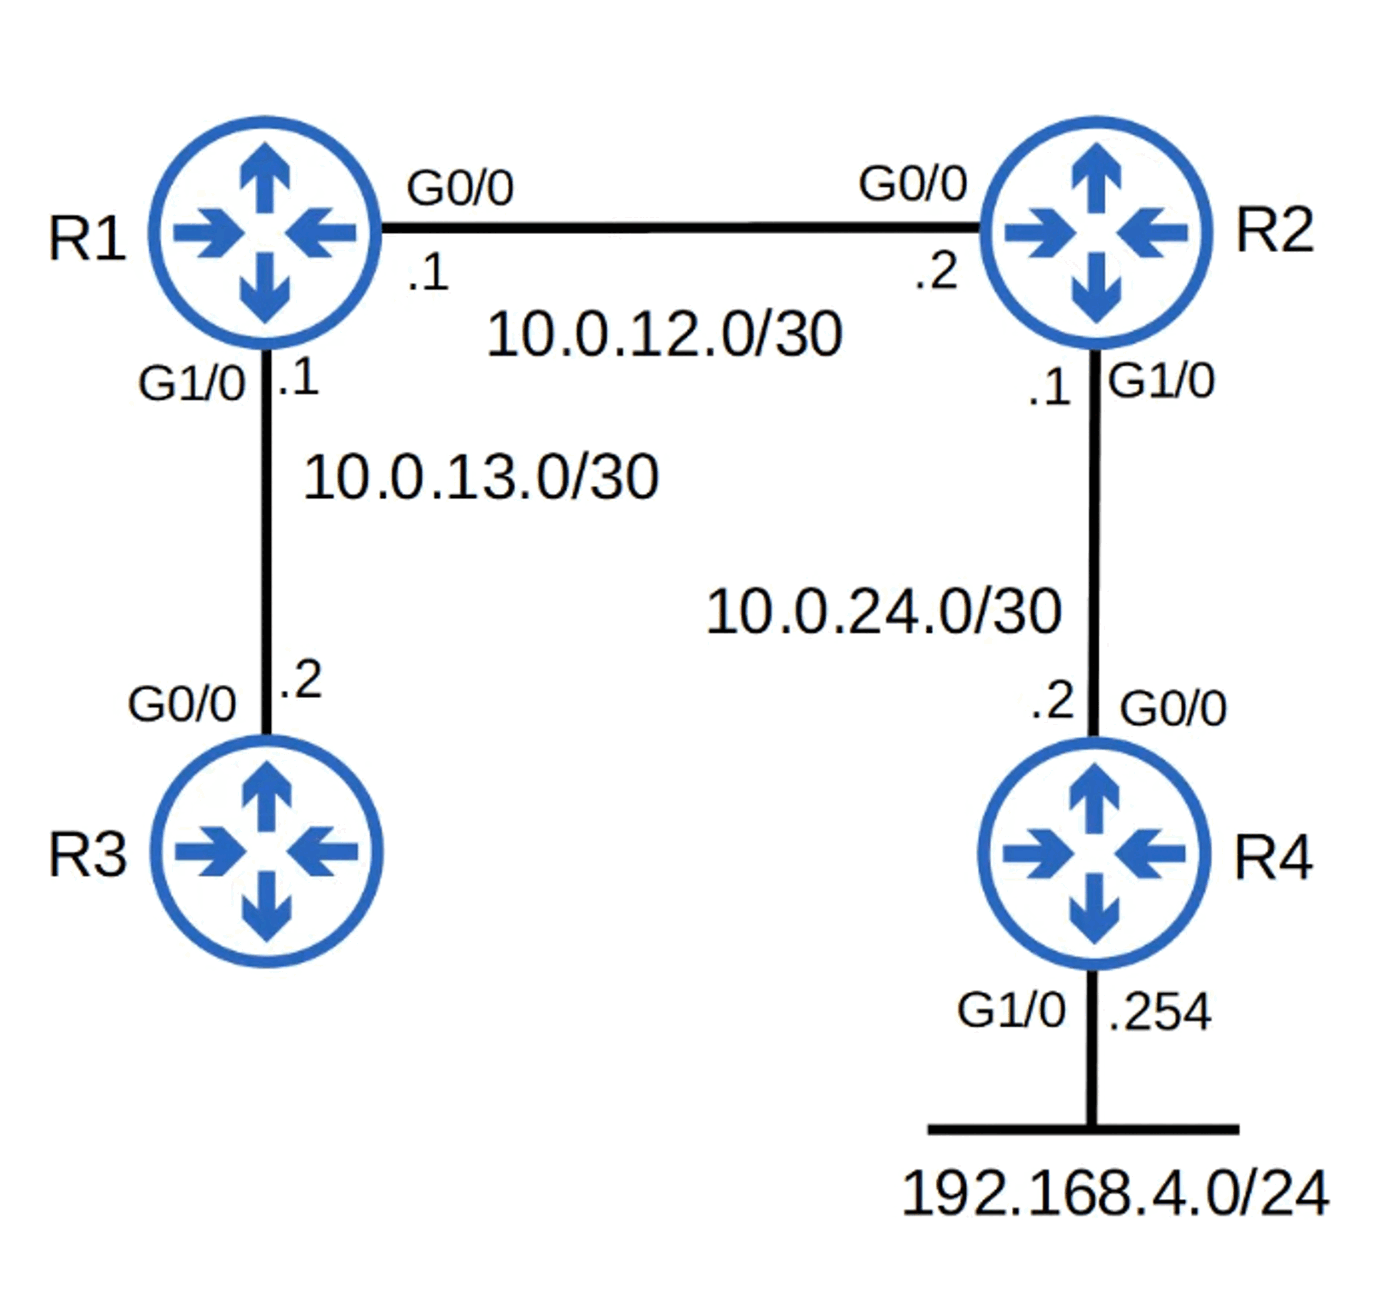
\includegraphics[keepaspectratio,alt={image}]{images/25-dynamicrouting/img-001.png}}
\end{figure}

\begin{itemize}
\tightlist
\item
  LAYER 3
\item
  Involves configuring a DYNAMIC ROUTING PROTOCOL on the ROUTER and
  letting the ROUTER take care of finding the best routes to DESTINATION
  NETWORKS.
\item
  Not Fixed (will adapt to changes in the LAN)
\end{itemize}

\begin{figure}
\centering
\pandocbounded{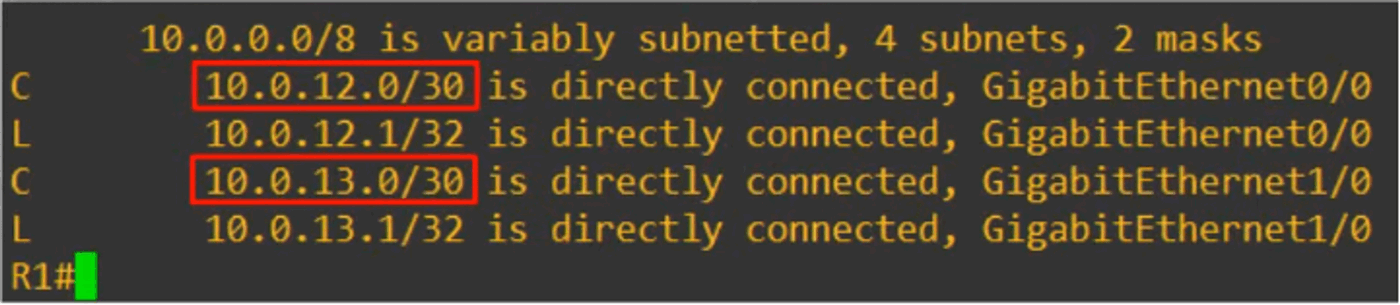
\includegraphics[keepaspectratio,alt={image}]{images/25-dynamicrouting/img-002.png}}
\end{figure}

A NETWORK ROUTE : A ROUTE to a NETWORK or SUBNET (Mask Length
\textless{} /32)

Ex: \textbf{10.0.12.0/30} and \textbf{10.0.13.0/30} (above) are NETWORK
ROUTES

A HOST ROUTE : A ROUTE to a specific HOST (/32 Mask)

Ex: \textbf{10.0.12.1/32} and \textbf{10.0.13.1/32} (above) are HOST
ROUTES

These two ROUTES were AUTOMATICALLY added to R1's G0/0 and G1/0s
INTERFACES

HOW DYNAMIC ROUTING WORKS ?

\begin{figure}
\centering
\pandocbounded{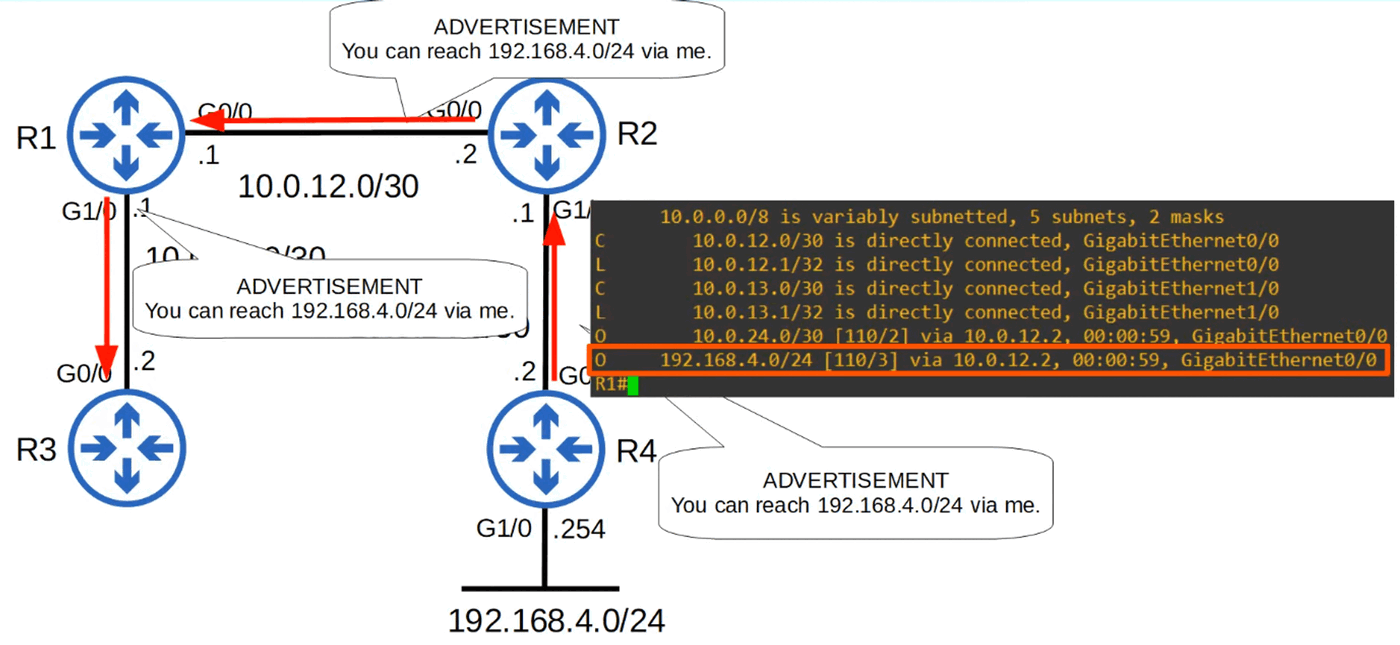
\includegraphics[keepaspectratio,alt={image}]{images/25-dynamicrouting/img-003.png}}
\end{figure}

(R4 ADVERTISES to R2 who ADVERTISES to R1 who ADVERTISES to R3 - They
add the NETWORK ROUTE to R4 in their ROUTE TABLE)

If the NETWORK ROUTE breaks, the ROUTE is DYNAMICALLY REMOVED from the
ROUTE TABLE

\begin{figure}
\centering
\pandocbounded{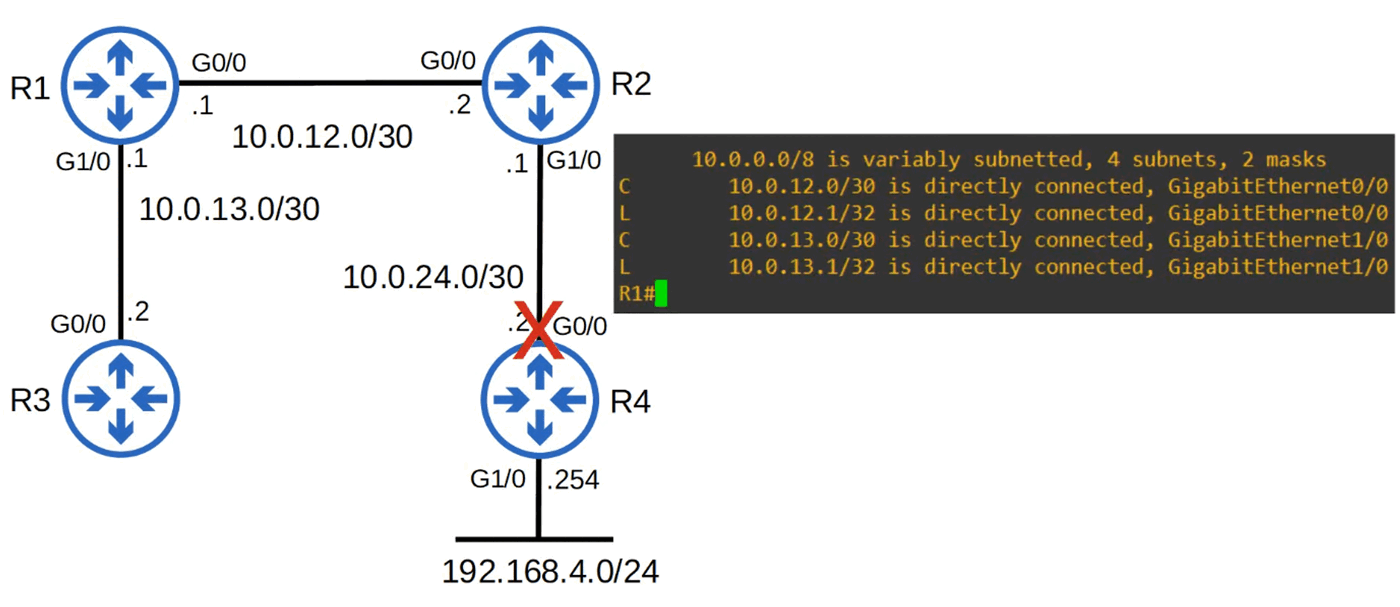
\includegraphics[keepaspectratio,alt={image}]{images/25-dynamicrouting/img-004.png}}
\end{figure}

(R1 removing the ROUTE to R4 from it's ROUTE TABLE)

IN STATIC ROUTING, a downed ROUTER will still have traffic passed to it.
The ROUTE TABLES are unchanged.

\begin{figure}
\centering
\pandocbounded{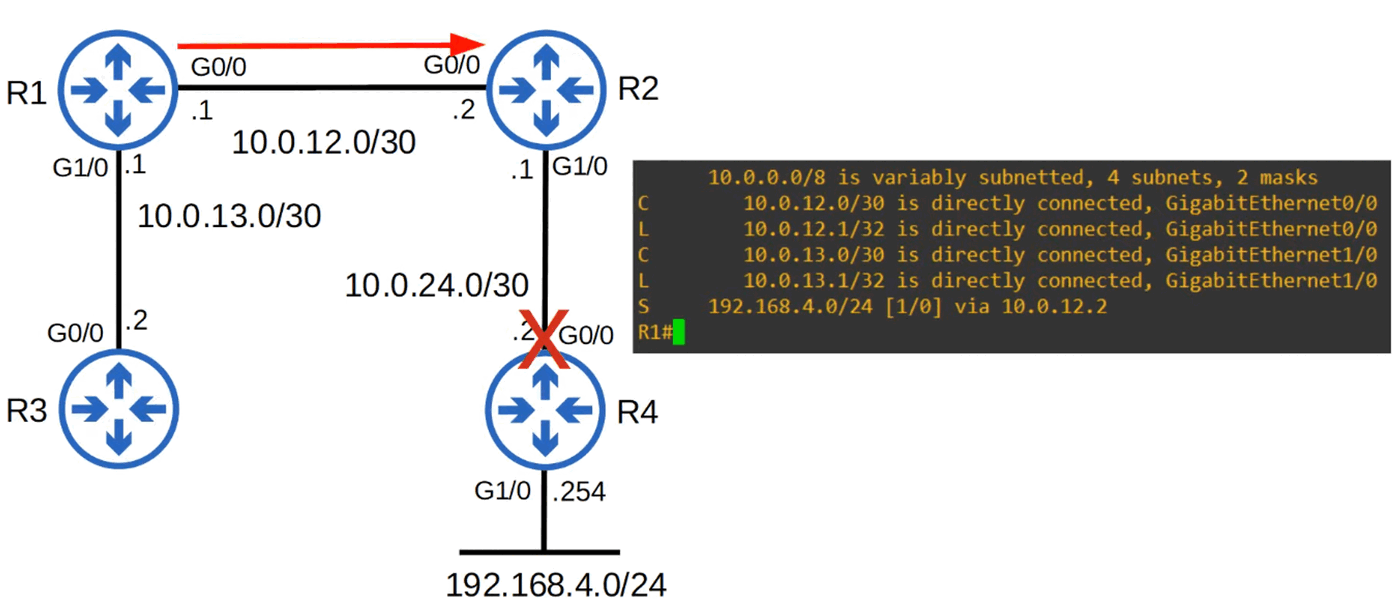
\includegraphics[keepaspectratio,alt={image}]{images/25-dynamicrouting/img-005.png}}
\end{figure}

(R1 has a STATIC ROUTE to R4 and passes traffic destined to it's NETWORK
regardless of status)

DYNAMIC ROUTING is good but still requires REDUNDANCY so we add another
connection between R3 and R4

\begin{figure}
\centering
\pandocbounded{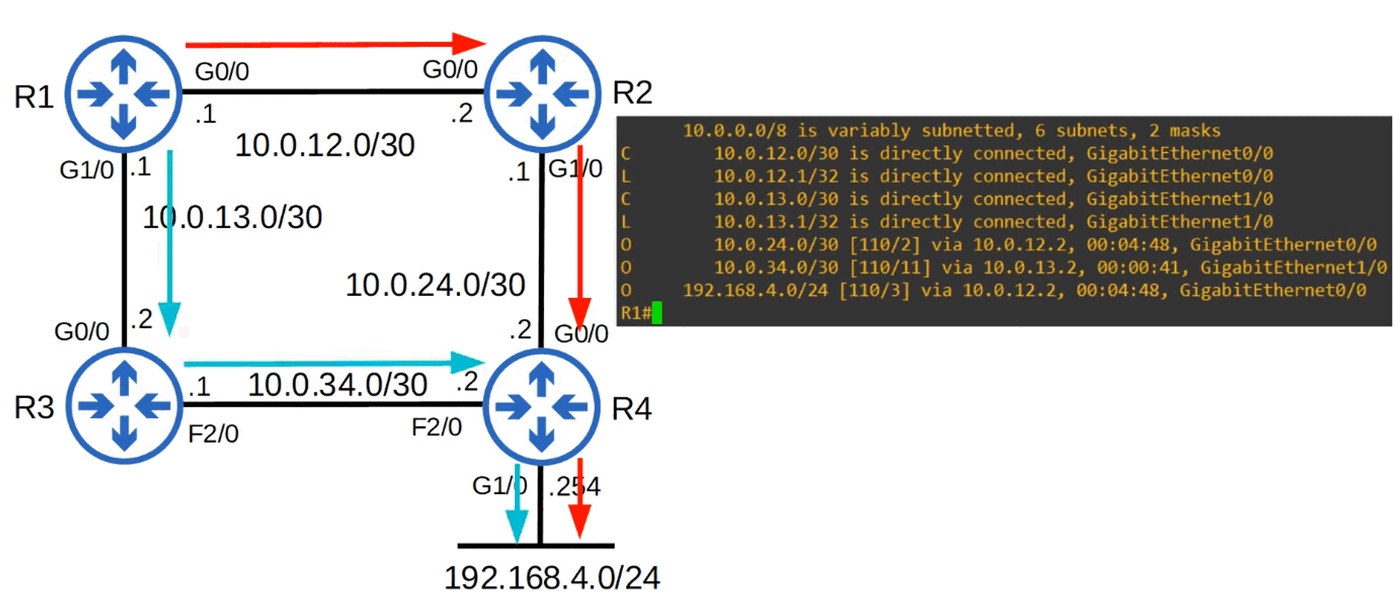
\includegraphics[keepaspectratio,alt={image}]{images/25-dynamicrouting/img-006.png}}
\end{figure}

(Secondary DYNAMIC ROUTE added to R4 from R1 via R3. ROUTE TABLE updated
appropriately)

A failure in the ROUTE, via R2 to R4's G0/0 INTERFACE, automatically
reroutes traffic via R3

\begin{figure}
\centering
\pandocbounded{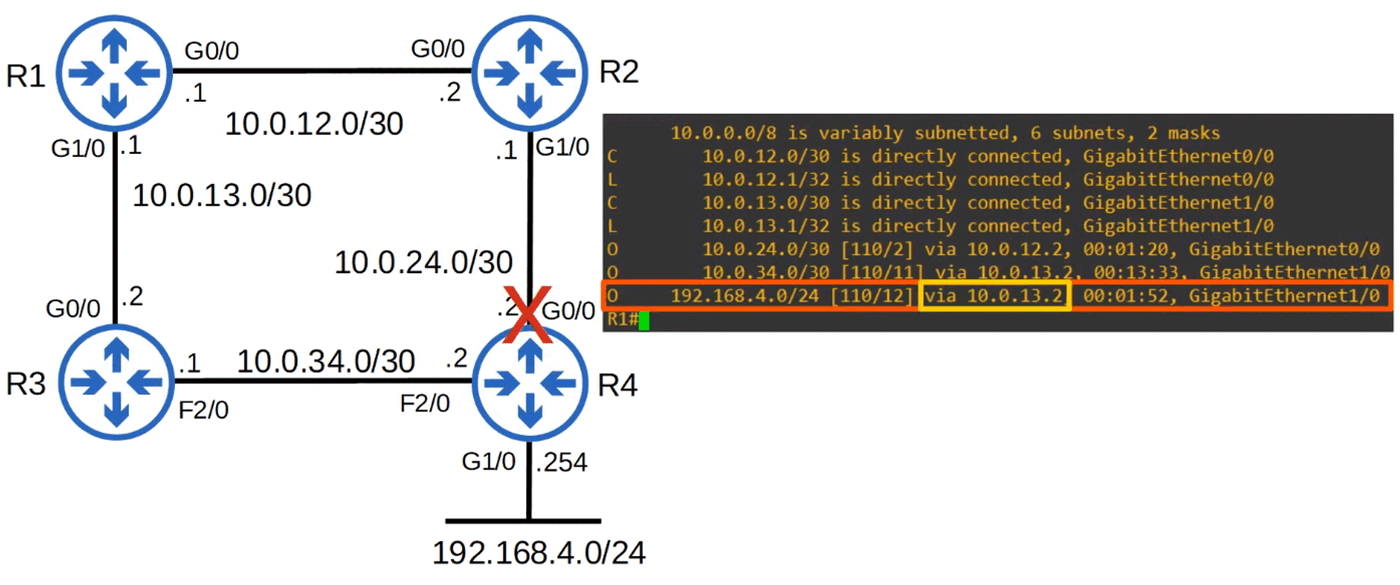
\includegraphics[keepaspectratio,alt={image}]{images/25-dynamicrouting/img-007.png}}
\end{figure}

Why does the path prefer using R2's path versus R3?

Because of COST ! This is similar to how SPANNING-TREE works (with
SWITCHES)

\section{Introduction to Dynamic Routing
Protocols}\label{introduction-to-dynamic-routing-protocols}

\begin{itemize}
\tightlist
\item
  ROUTERS can use DYNAMIC ROUTING PROTOCOLS to ADVERTISE information
  about the ROUTES they know to OTHER ROUTES
\item
  They form `ADJACENCIES' / `NEIGHBOR RELATIONSHIPS' / `NEIGHBORSHIPS'
  with ADJACENT ROUTERS to exchange this information
\item
  If multiple ROUTES to a DESTINATION are learned, the ROUTER determines
  which ROUTE is SUPERIOR and adds it to the ROUTING TABLE. It uses the
  `METRIC' of the ROUTE to decide which is superior (lower metric =
  superior)
\end{itemize}

\section{Types of Dynamic Routing
Protocols}\label{types-of-dynamic-routing-protocols}

DYNAMIC ROUTING PROTOCOLS can be divided into TWO main categories:

\begin{itemize}
\tightlist
\item
  IGP (Interior Gateway Protocol)
\item
  EGP (Exterior Gateway Protocol)
\end{itemize}

\section{Igp}\label{igp}

\begin{itemize}
\tightlist
\item
  Used to SHARE ROUTES within a single \emph{autonomous system} (AS),
  which is a single organization (ie: a company)
\end{itemize}

\begin{figure}
\centering
\pandocbounded{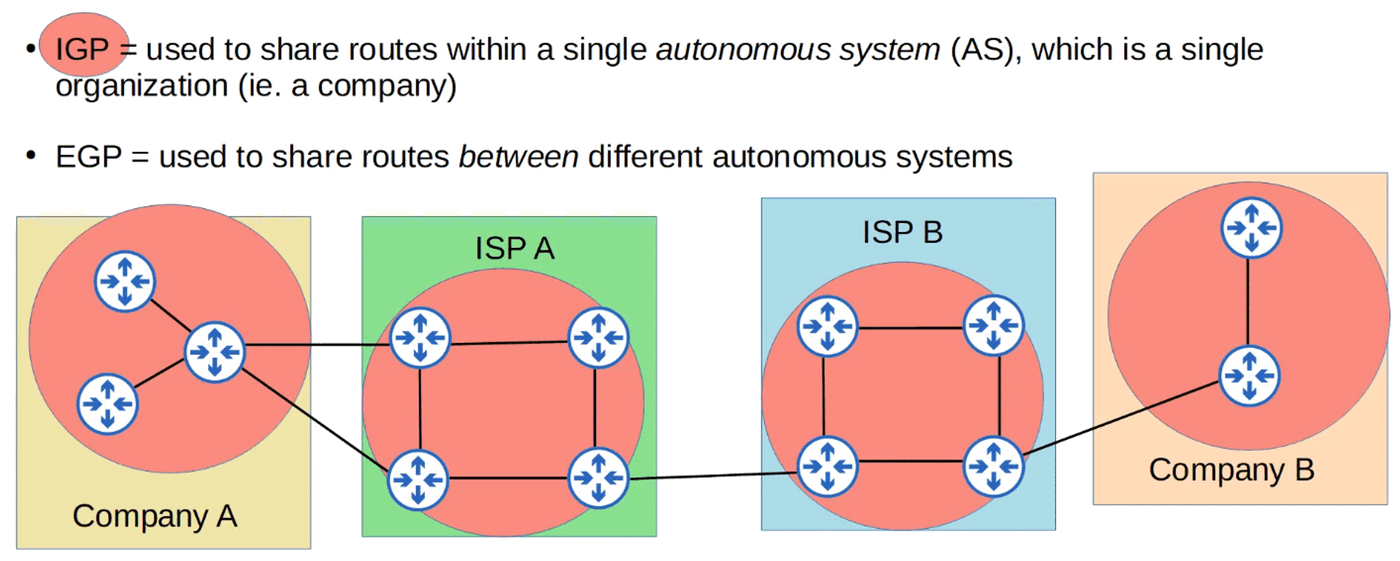
\includegraphics[keepaspectratio,alt={image}]{images/25-dynamicrouting/img-008.png}}
\end{figure}

\section{Egp}\label{egp}

\begin{itemize}
\tightlist
\item
  Used to SHARE ROUTES \emph{between} different \emph{autonomous systems
  (AS)}
\end{itemize}

\begin{figure}
\centering
\pandocbounded{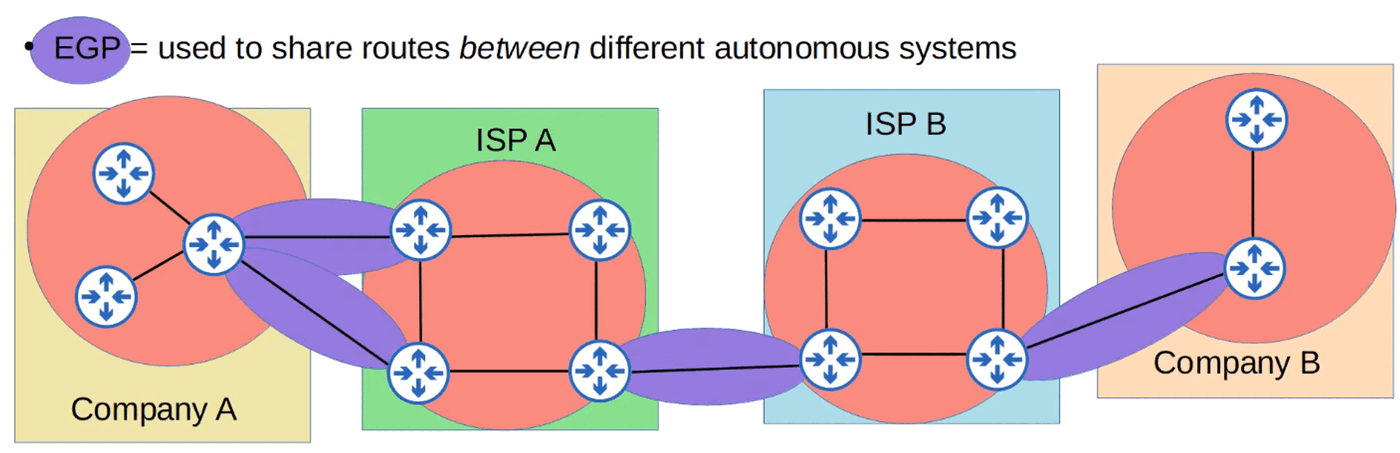
\includegraphics[keepaspectratio,alt={image}]{images/25-dynamicrouting/img-009.png}}
\end{figure}

Algorithms used for IGP and EGP and the PROTOCOL for each

\begin{figure}
\centering
\pandocbounded{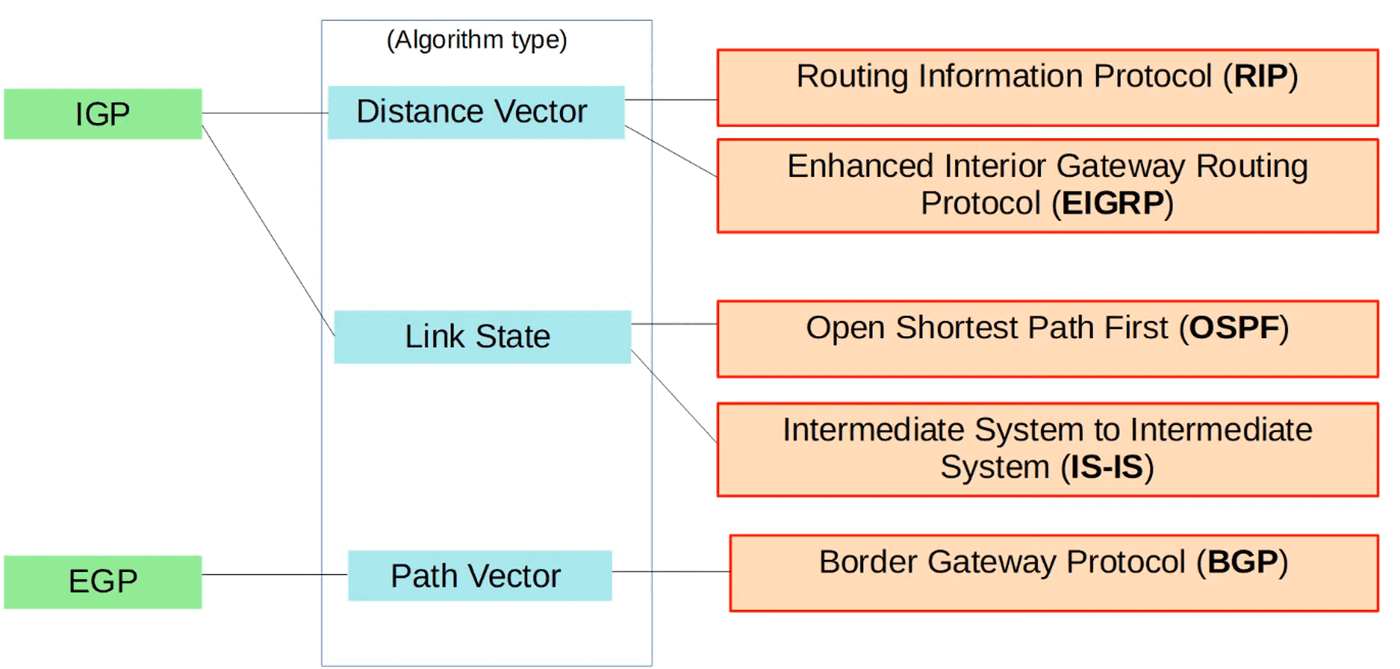
\includegraphics[keepaspectratio,alt={image}]{images/25-dynamicrouting/img-010.png}}
\end{figure}

YOU MUST MEMORIZE WHICH ALGORITHM IS USED FOR EACH PROTOCOL FOR THE
CCNA!

\section{Distance Vector Routing
Protocols}\label{distance-vector-routing-protocols}

\begin{itemize}
\item
  Called DISTANCE VECTOR because the ROUTERS only learn the `distance'
  (METRIC) and `vector' (DIRECTION, NEXT-HOP ROUTER) of each ROUTE
\item
  DISTANCE VECTOR PROTOCOLS were invented before LINK STATE PROTOCOLS
\item
  Early examples are RIPv1 and Cisco's IGRP (which was updated to EIGRP)
\item
  DISTANCES VECTOR PROTOCOLS operate by sending the following to their
  directly connection neighbors:

  \begin{itemize}
  \tightlist
  \item
    Their KNOWN DESTINATION networks
  \item
    Their METRIC to reach their KNOWN DESTINATION networks
  \end{itemize}
\item
  This METHOD of sharing ROUTE information is often called
  \textbf{\emph{`routing by rumor'}}

  \begin{itemize}
  \tightlist
  \item
    \textbf{\emph{`routing by rumor'}} = because the ROUTER doesn't know
    about the NETWORK beyond it's NEIGHBOURS. It only knows the
    information that the NEIGHBOURS tell it.
  \end{itemize}
\end{itemize}

\begin{figure}
\centering
\pandocbounded{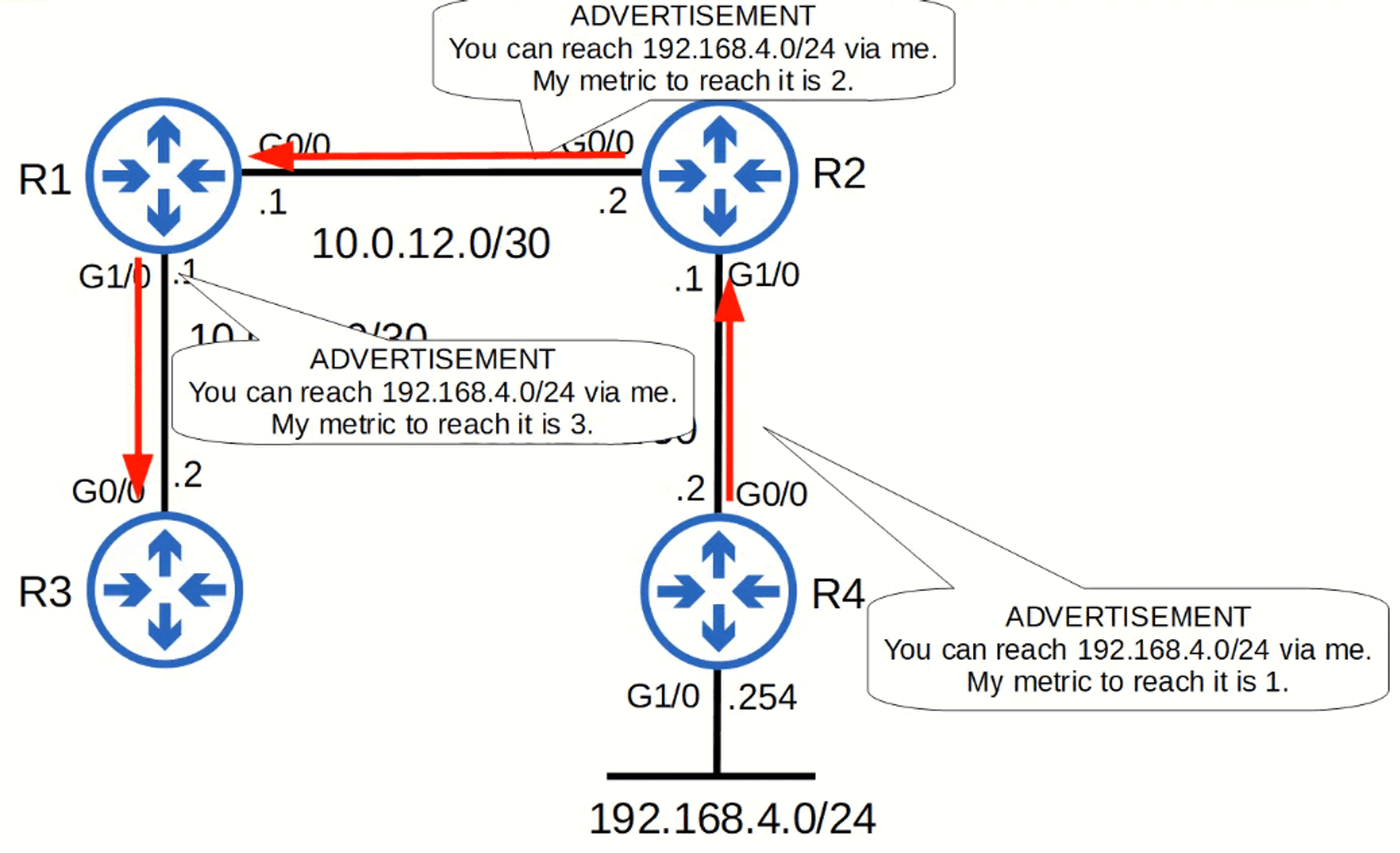
\includegraphics[keepaspectratio,alt={image}]{images/25-dynamicrouting/img-011.png}}
\end{figure}

\section{Dynamic Routing Protocol
Metrics}\label{dynamic-routing-protocol-metrics}

\begin{itemize}
\tightlist
\item
  A ROUTER'S ROUTE TABLE contains the BEST ROUTE to each DESTINATION
  NETWORK it knows about
\end{itemize}

If a ROUTER using a DYNAMIC ROUTING PROTOCOL learns TWO different routes
to the same DESTINATION, how does it determine which is \textbf{`best'}
?

It uses the METRIC value of the ROUTES to determine which is BEST.

A lower METRIC = BETTER! (just like STP)

EACH ROUTING PROTOCOL uses a different METRIC to determine which ROUTE
is best

\begin{figure}
\centering
\pandocbounded{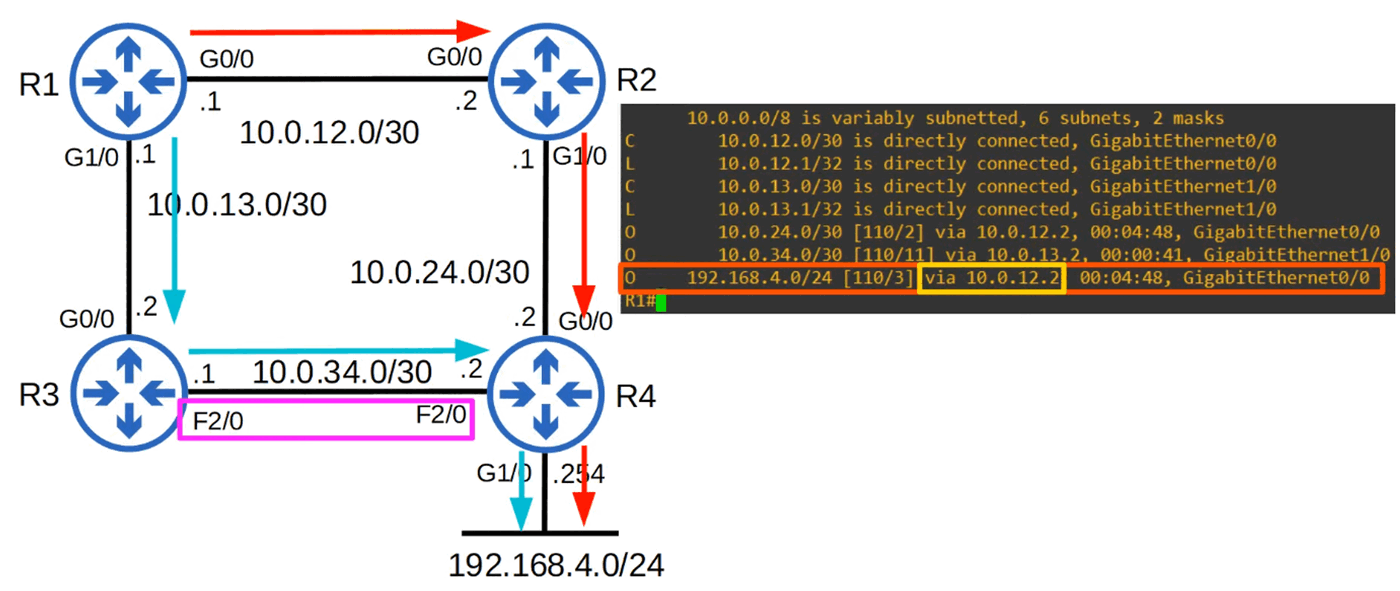
\includegraphics[keepaspectratio,alt={image}]{images/25-dynamicrouting/img-012.png}}
\end{figure}

The above choose the RED PATH because the ``cost'', using R3 F2/0 and R4
F2/0 (FastEthernet) is HIGHER than the R2 G1/0 and R4 G0/0
(GigabyteEthernet)

What if BOTH connections were GigabyteEthernet? (ie: the same METRIC
value)

\begin{figure}
\centering
\pandocbounded{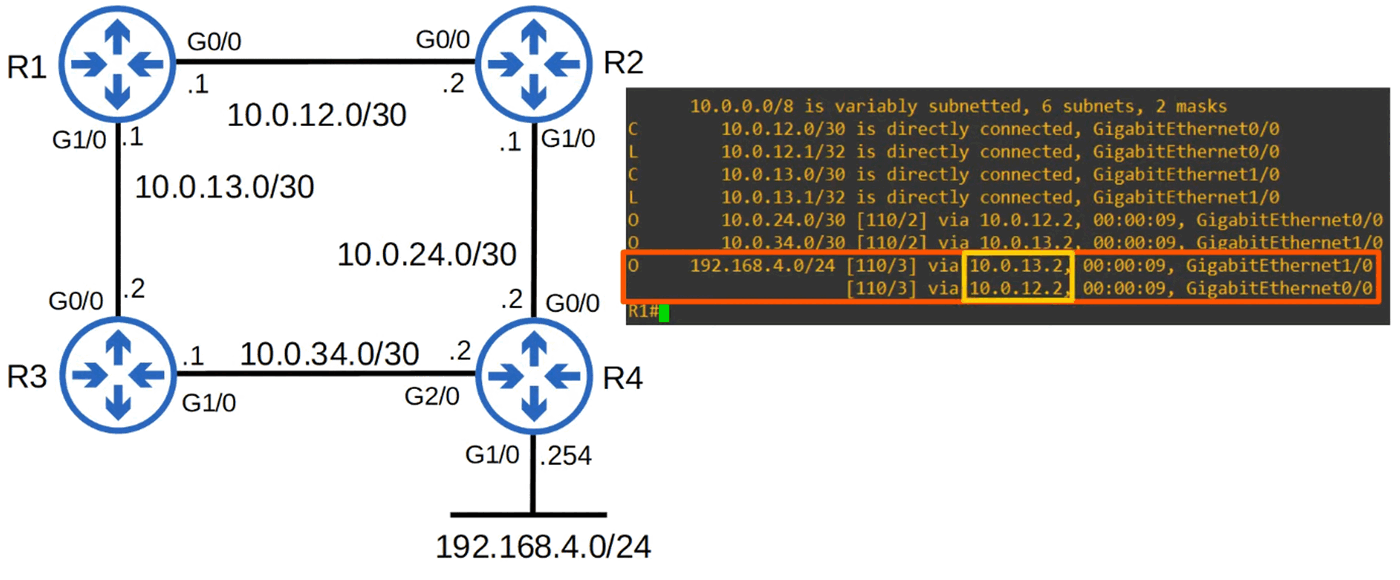
\includegraphics[keepaspectratio,alt={image}]{images/25-dynamicrouting/img-013.png}}
\end{figure}

BOTH ROUTES are added to the ROUTE TABLE

So \ldots{}

If a ROUTER learns TWO (or more) ROUTES via the same ****ROUTING
PROTOCOL to the same DESTINATION (same network address, same subnet
mask) with the same METRIC, both will be added to the routing table.
Traffic will be LOAD-BALANCED over both ROUTES

\begin{figure}
\centering
\pandocbounded{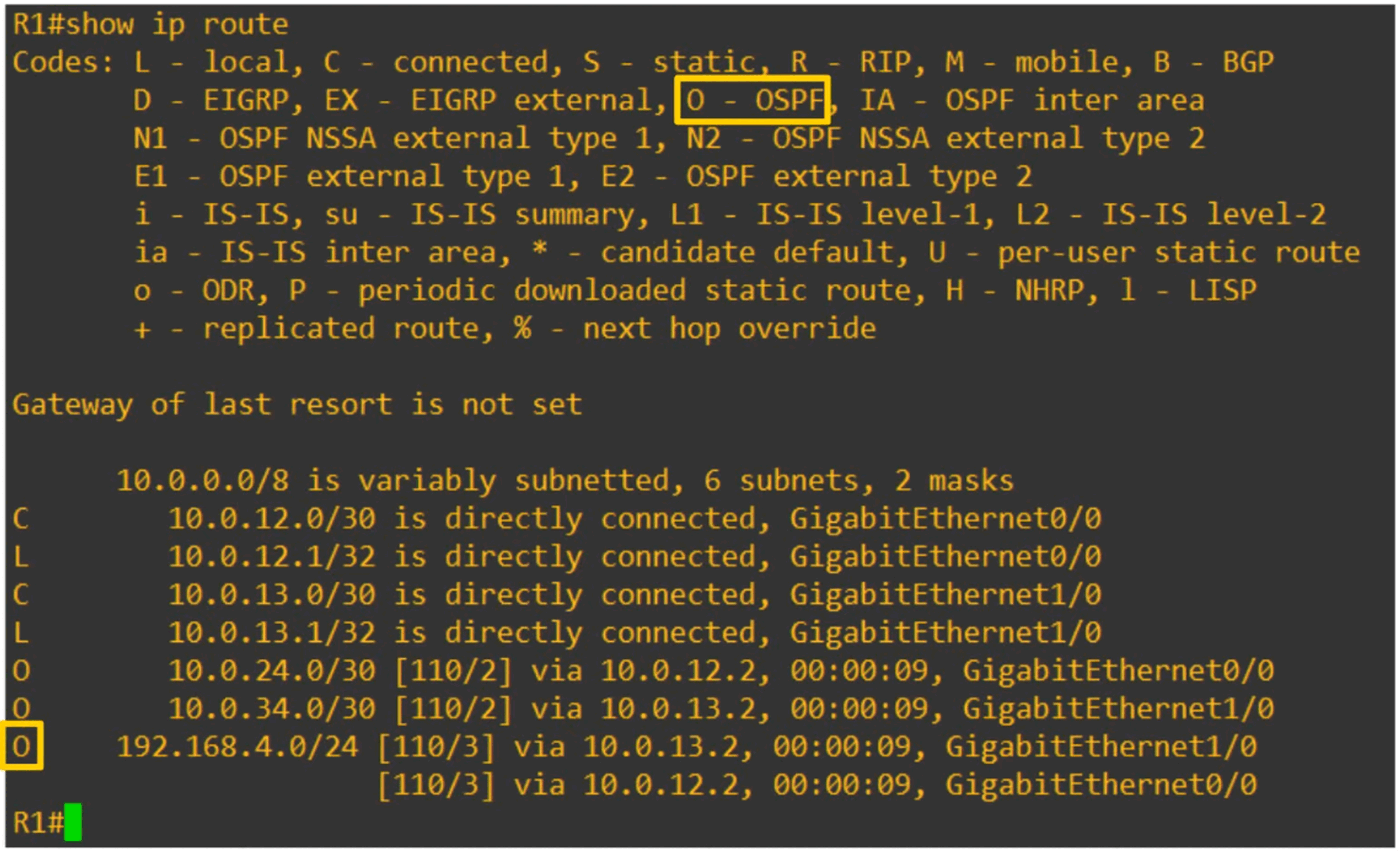
\includegraphics[keepaspectratio,alt={image}]{images/25-dynamicrouting/img-014.png}}
\end{figure}

``O'' = OSPF PROTOCOL (next to ROUTES)

{[}110/3{]} :

\begin{itemize}
\tightlist
\item
  the ``3'' part is the METRIC.
\item
  the ``110'' part is ADMINISTRATIVE DISTANCE (covered later)
\end{itemize}

Since BOTH ROUTES share the same METRIC, this is called ECMP (EQUAL COST
MULTI-PATH)

You can have ECMP with STATIC ROUTES, as well (they don't use METRIC,
however)

\section{Summary of Different
Metrics}\label{summary-of-different-metrics}

\begin{figure}
\centering
\pandocbounded{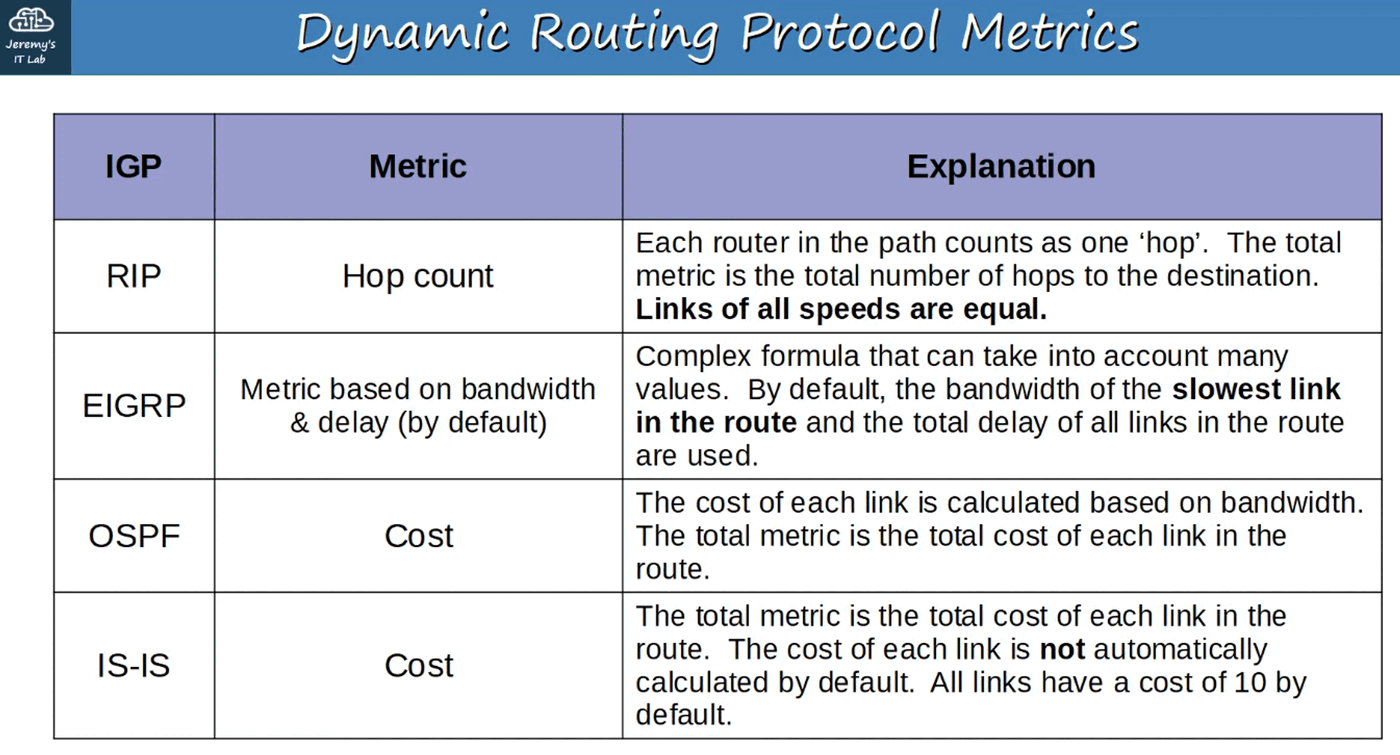
\includegraphics[keepaspectratio,alt={image}]{images/25-dynamicrouting/img-015.png}}
\end{figure}

(IS-IS won't be covered in detail)

\section{Example}\label{example}

\begin{figure}
\centering
\pandocbounded{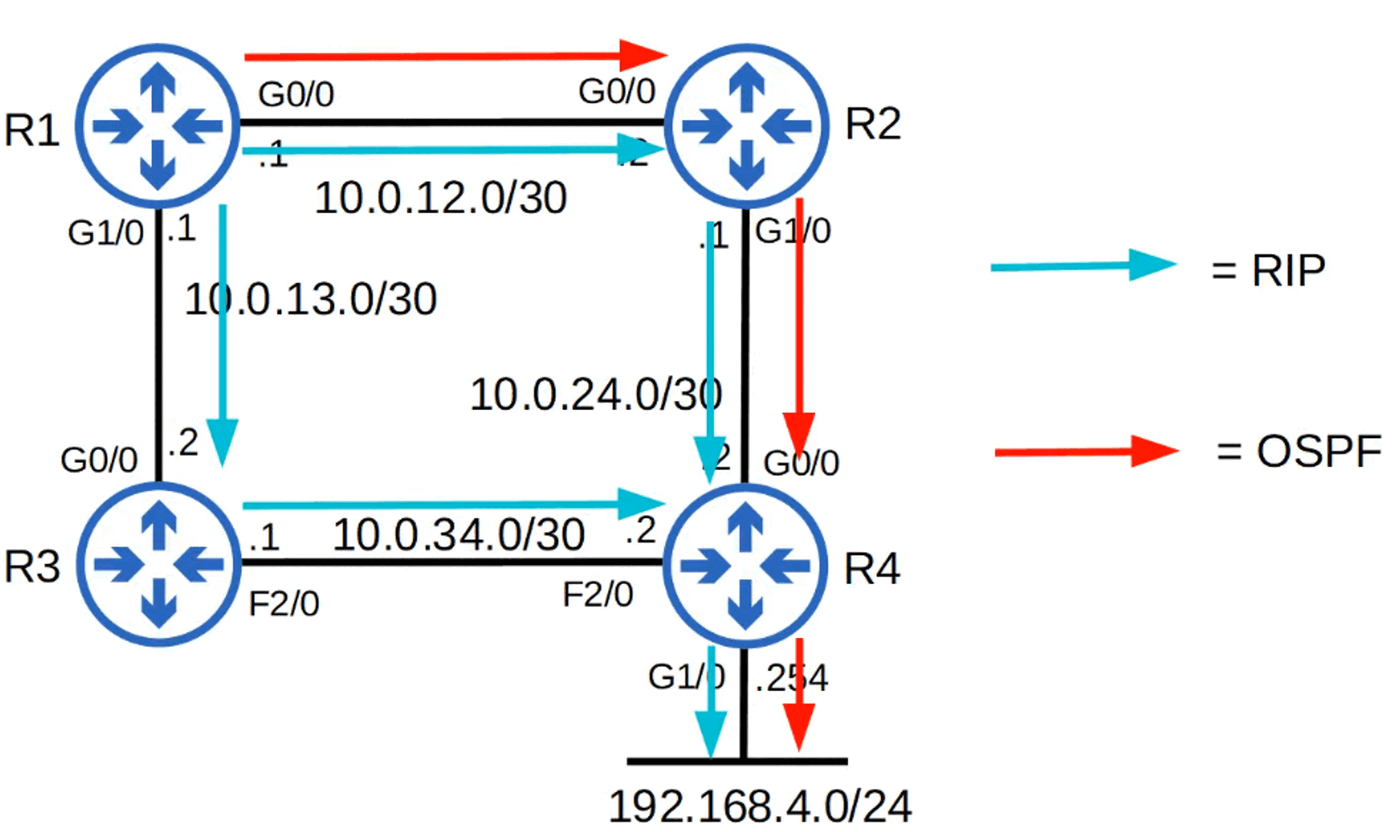
\includegraphics[keepaspectratio,alt={image}]{images/25-dynamicrouting/img-016.png}}
\end{figure}

Using RIP, both ROUTES would be put in R1's ROUTE TABLE

Using OSPF, only the ROUTE from R1 \textgreater{} R2 \textgreater{} R4
would be added to R1's ROUTE TABLE because of the TOTAL COST of each
link.

However, BOTH METRICS are trying to achieve the same thing :

To let the ROUTER select the BEST ROUTE to the DESTINATION

\section{Administrative Distance}\label{administrative-distance}

\begin{itemize}
\item
  In MOST cases, a company will only use a single IGP - usually OSPF or
  EIGRP
\item
  However, in some RARE cases, they might use TWO.

  \begin{itemize}
  \tightlist
  \item
    Ex: If TWO companies connect their networks to share information,
    TWO different ROUTING PROTOCOLS might be in use.
  \end{itemize}
\item
  METRIC is used to compare ROUTES learned via the same ROUTING PROTOCOL
\item
  Different ROUTING PROTOCOLS use totally different METRICS, so they
  cannot be compared

  \begin{itemize}
  \tightlist
  \item
    An OSPF ROUTE to 192.168.4.0/24 might have a METRIC of 30, while an
    EIGRP ROUTE to the same DESTINATION has a METRIC of 33280. Which
    ROUTE is better? Which route should the ROUTER put in the ROUTE
    TABLE ?
  \end{itemize}
\item
  The \textbf{ADMINISTRATIVE DISTANCE (AD)}, is used to determine which
  ROUTING PROTOCOL is preferred.

  \begin{itemize}
  \tightlist
  \item
    A LOWER AD is preferred, and indicates that the ROUTING PROTOCOL is
    considered more `trustworthy' (more likely to select good ROUTES)
  \end{itemize}
\end{itemize}

\section{Administrative Distance
Numbers}\label{administrative-distance-numbers}

\begin{figure}
\centering
\pandocbounded{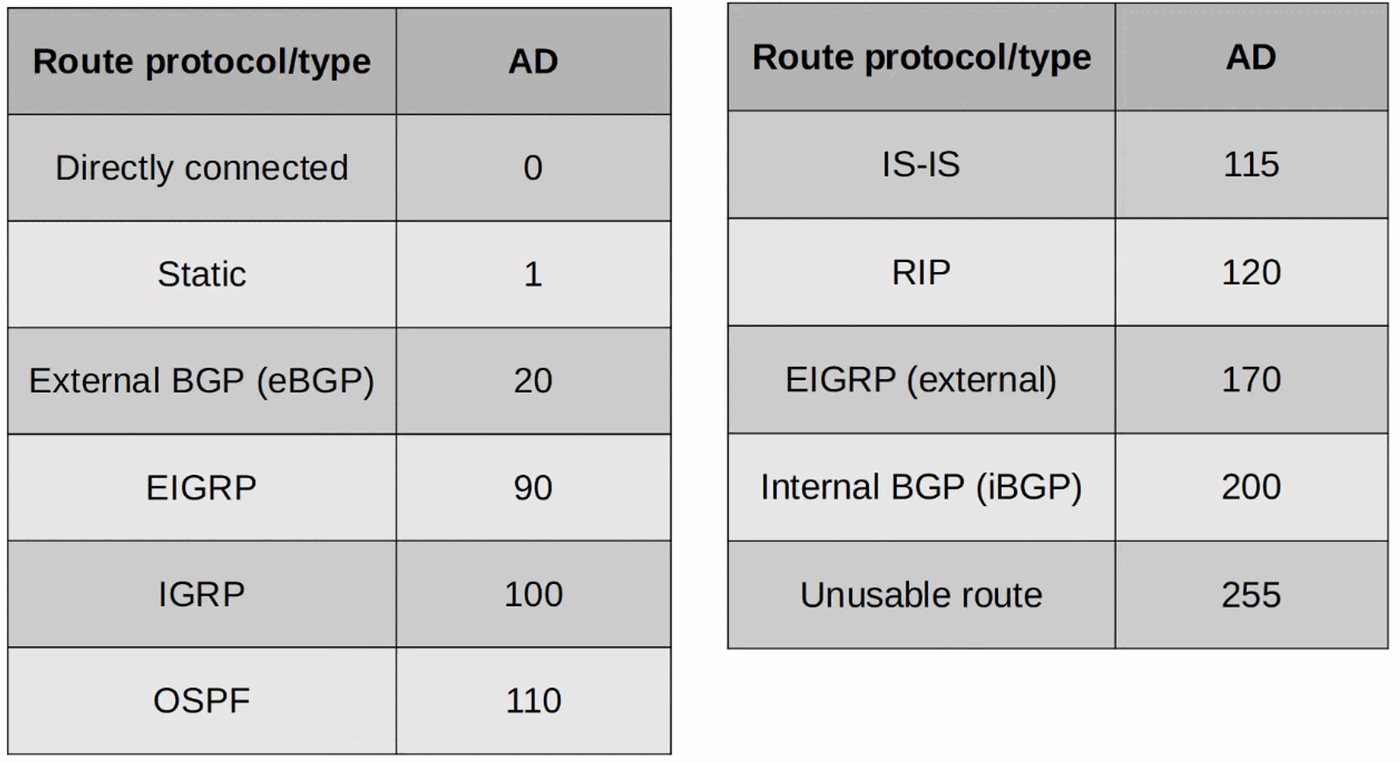
\includegraphics[keepaspectratio,alt={image}]{images/25-dynamicrouting/img-017.png}}
\end{figure}

(USE THE FLASHCARDS TO MEMORIZE THESE)

IF the ADMINISTRATIVE DISTANCE is 255, the ROUTER does not believe the
SOURCE of that ROUTE and does not install the ROUTE in the ROUTING
TABLE!

\begin{figure}
\centering
\pandocbounded{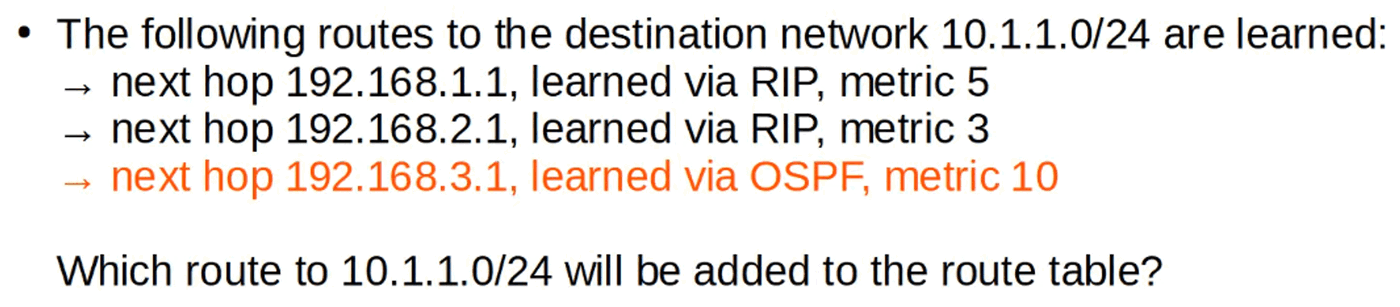
\includegraphics[keepaspectratio,alt={image}]{images/25-dynamicrouting/img-018.png}}
\end{figure}

METRIC is used to COMPARE ROUTES learned from the SAME ROUTING PROTOCOL

However, before comparing METRICS, AD is used to select the BEST ROUTE

Therefore, the BEST ROUTE is :

``next hop 192.168.3.1, learned via OSPF (lower AD than RIP), metric
10''

\begin{itemize}
\tightlist
\item
  You can CHANGE the AD of a ROUTING PROTOCOL (This will be demonstrated
  in the lecture for OSPF CONFIGURATION)
\item
  You can also change the AD of a STATIC ROUTE:
\end{itemize}

\begin{figure}
\centering
\pandocbounded{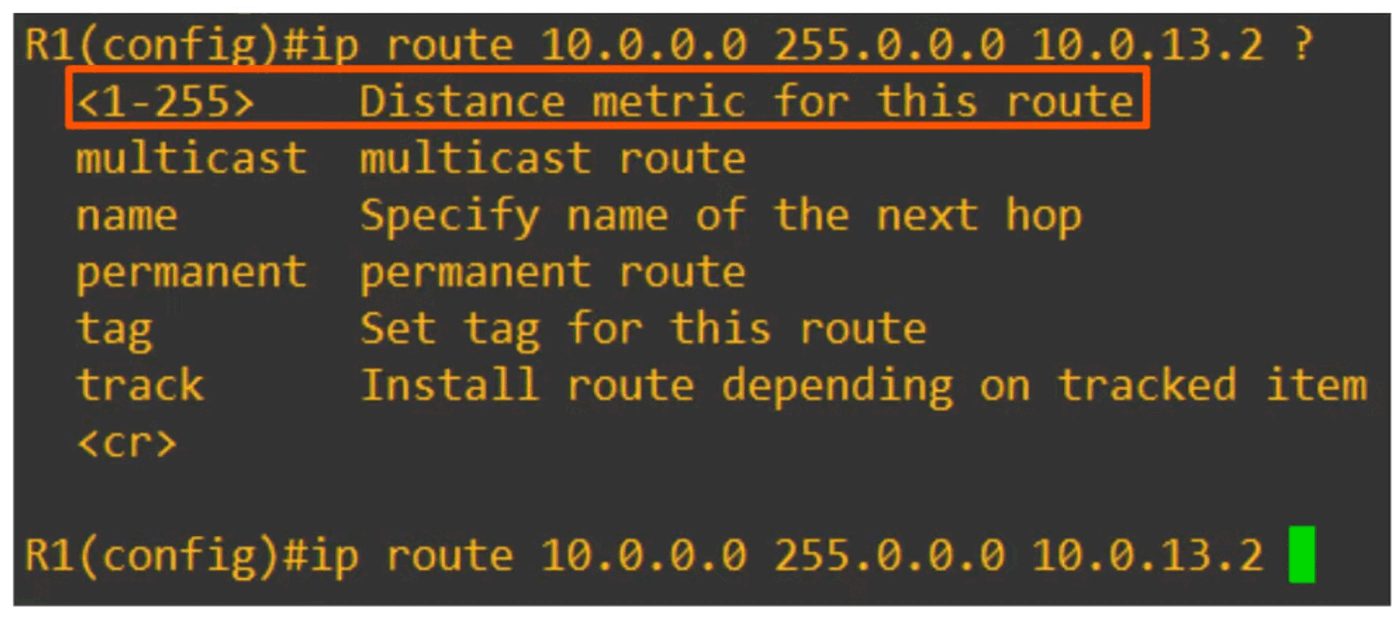
\includegraphics[keepaspectratio,alt={image}]{images/25-dynamicrouting/img-019.png}}
\end{figure}

\begin{figure}
\centering
\pandocbounded{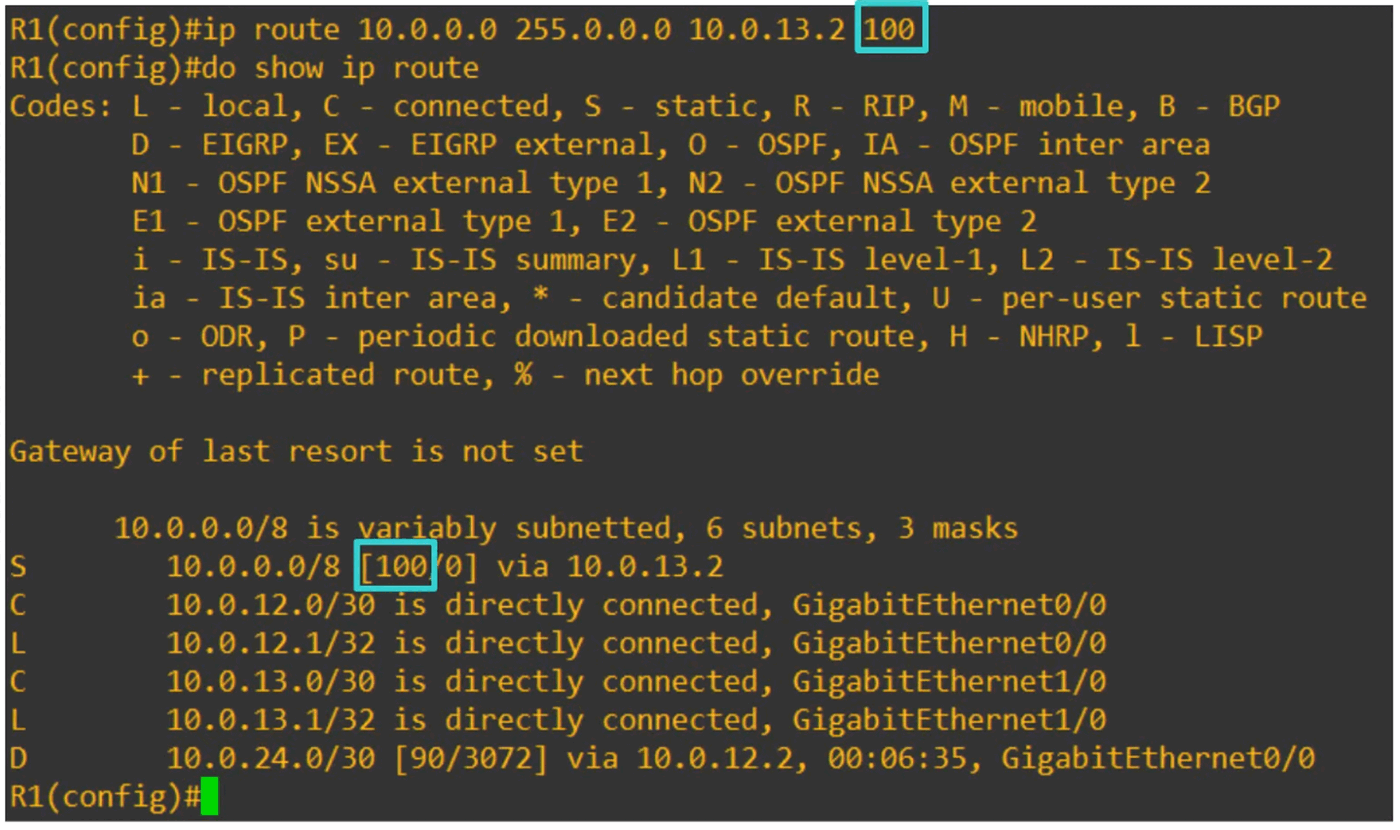
\includegraphics[keepaspectratio,alt={image}]{images/25-dynamicrouting/img-020.png}}
\end{figure}

WHY WOULD YOU WANT TO DO THIS?

\section{Floating Static Routes}\label{floating-static-routes}

\begin{itemize}
\tightlist
\item
  By CHANGING the AD of a STATIC ROUTE, you can make it less preferred
  than ROUTES learned by a DYNAMIC ROUTING PROTOCOL to the same
  DESTINATION (make sure the AD is HIGHER than the ROUTING PROTOCOL's
  AD!)
\item
  This kind of ROUTE is called a `FLOATING STATIC ROUTE'
\item
  The ROUTE will be inactive (not in the ROUTING TABLE) unless the ROUTE
  learned by the DYNAMIC ROUTING PROTOCOL is removed.

  \begin{itemize}
  \tightlist
  \item
    \textbf{Ex:} The remote ROUTER stops ADVERTISING it for some reason,
    or an INTERFACE failure causes an ADJACENCY with a NEIGHBOR to be
    lost.
  \end{itemize}
\end{itemize}

\section{Link State Routing
Protocols}\label{link-state-routing-protocols}

\begin{itemize}
\tightlist
\item
  When using a LINK STATE ROUTING PROTOCOL, every ROUTER creates a
  `connectivity map' of the NETWORK
\item
  To allow this, each ROUTER ADVERTISES information about its INTERFACES
  (connected NETWORKS) to its NEIGHBOURS. These ADVERTISEMENTS are
  passed along to the other ROUTERS, until all ROUTERS in the NETWORK
  develop the same map of the NETWORK
\item
  Each ROUTER independently uses this MAP to calculate the BEST ROUTES
  to each DESTINATION
\item
  LINK STATE PROTOCOLS use more resources (CPU) on the ROUTER, because
  MORE information is shared.
\item
  However, LINK STATE PROTOCOLS tend to be FASTER in reacting to CHANGES
  in the NETWORK than DISTANCES VECTOR PROTOCOLS
\end{itemize}
